\documentclass[dvisvgm,hypertex,aspectratio=169]{beamer}
\usefonttheme{serif}

%\usepackage[utf8]{inputenc}
%\usepackage[T1]{fontenc}

%\usepackage[draft]{animate}
\usepackage[final]{animate}
\usepackage{ifthen}


%\usepackage{pythontex} % <--
\usepackage{graphicx}


\usepackage{tikz}
\usepackage{pgfplots}
\usepackage{pgfplotstable}
\pgfplotsset{compat=1.16}
\usetikzlibrary{calc}
\usetikzlibrary{decorations.pathmorphing,patterns}
\usepackage{amsmath}


%%%%%%%%%%%%%%%%%%%%%%%%%%%%%%%%%%%%%%%%%%%%%%%%%%%%%%%%%%%%%%%%%%%%%%%%%%%%%%% 
% Define footer
\usepackage{ccicons}

\makeatletter
\setbeamertemplate{footline}
{
  \leavevmode%
  \hbox{%
  %\begin{beamercolorbox}[wd=.333333\paperwidth,ht=2.25ex,dp=1ex,center]{title in head/foot}%
    %\usebeamerfont{title in head/foot}\insertsubsection
  %\end{beamercolorbox}%
  %\begin{beamercolorbox}[wd=.333333\paperwidth,ht=2.25ex,dp=1ex,right]{date in head/foot}%
  %  \usebeamerfont{date in head/foot}\insertshortdate{}\hspace*{2em}
  %  \insertframenumber{} / \inserttotalframenumber\hspace*{2ex} 
  %\end{beamercolorbox}}%
  %\vskip0pt%
  \begin{beamercolorbox}[wd=.92\paperwidth,ht=2.25ex,dp=1ex,right]{author in head/foot}%
    \usebeamerfont{author in head/foot}\insertauthor
  \end{beamercolorbox}%
  \begin{beamercolorbox}[wd=.08\paperwidth,ht=2.25ex,dp=1ex,right]{date in head/foot}%
    \ccbysa
  \end{beamercolorbox}}%
  \vskip0pt%
}
\makeatother
%%%%%%%%%%%%%%%%%%%%%%%%%%%%%%%%%%%%%%%%%%%%%%%%%%%%%%%%%%%%%%%%%%%%%%%%%%%%%%%


\author{\href{mailto:kjartan@tec.mx}{kjartan@tec.mx}}

\begin{document}

\section{Create animation}

  \def\tend{30}
  \def\nframes{24}
  \def\nsamples{200}
  \def\wexpstart{-2}
  \def\wexpend{1}
  \def\ttau{1}
  
\begin{frame}[label=A]{First-order Bode plot}
      \begin{center}
        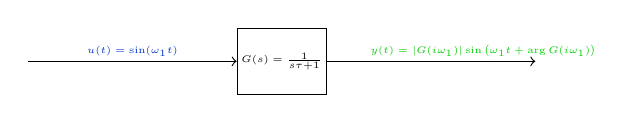
\begin{tikzpicture}[scale=0.7, transform shape,]
          \tiny
          \node[draw, minimum width=14mm, minimum height=12mm] (sys) {$G(s)=\frac{1}{s\tau + 1}$};
          \node[coordinate, left of=sys, node distance=46mm] (input) {};
          \node[coordinate, right of=sys, node distance=46mm] (output) {};
          \draw[->] (input) -- node[ above] { $\textcolor{blue!80!green}{u(t)=\sin(\omega_1 t)}$} (sys);
          \draw[->] (sys) -- node[near end, above] { $\textcolor{green!80!black}{y(t)=|G(i\omega_1)|\sin\big(\omega_1 t + \arg G(i\omega_1)\big)}$} (output);
        \end{tikzpicture}
      \end{center}
      \begin{center}
        \begin{animateinline}[controls, loop, palindrome]{4}
          \multiframe{\nframes}{n=0+1}{
            
            \pgfmathsetmacro{\wexp}{\wexpstart + (\wexpend-\wexpstart)/\nframes*\n}
            \pgfmathsetmacro{\ww}{pow(10, \wexp)}
            \pgfmathsetmacro{\wstart}{pow(10, \wexpstart)}
            \pgfmathsetmacro{\wend}{pow(10, \wexpend)}
            \pgfmathsetmacro{\gain}{1/sqrt(pow(\ttau*\ww,2) + 1)}
            \pgfmathsetmacro{\phshift}{-atan2(\ttau*\ww,1)}

            \begin{tikzpicture}[scale=0.5, transform shape]

            \begin{loglogaxis} [
            width=7cm,
            height=5cm,
            ylabel=$|G|$,
            %xticklabels=\empty,
            xtick={0.01, 0.1, 1, 10},
            xticklabels={$\frac{0.01}{\tau}$, $\frac{0.1}{\tau}$, $\frac{1}{\tau}$, $\frac{10}{\tau}$}, 
            grid=both,
            minor y tick num=9,
            % extra y ticks={.5}, % how to convert to fixed point tick label ?
            % extra y tick style={log identify minor tick positions=true},
            every major grid/.style={red, opacity=0.5},
            ymin=0.01, ymax=2,
            xmin = 0.01, xmax=10,
            ]
            \addplot+[thick, orange!80!black, no marks, domain=\wstart:\wend, samples=100]
                  {1/sqrt(pow((\ttau*\x),2) + 1)};
            \draw[black!90, ] (axis cs: \ww, 0.01) -- (axis cs: \ww, 10);
            \node[magenta!80!black, circle, draw, inner sep=2pt, thick,] at (axis cs: \ww, \gain) {};
          \end{loglogaxis}
          \begin{semilogxaxis} [
            xlabel=$\omega$,
            ylabel=$\arg G$,
            xshift = 8cm, 
            width=7cm,
            height=5cm,
            grid=both,
            ytick={0, -90},
            ymin=-90, ymax = 0,
            xtick={0.01, 0.1, 1, 10},
            xticklabels={$\frac{0.01}{\tau}$, $\frac{0.1}{\tau}$, $\frac{1}{\tau}$, $\frac{10}{\tau}$},
            xmin = 0.01, xmax = 10,
            minor y tick num=2,
            every major grid/.style={red, opacity=0.5},
            %legend entries={Bessel filter, Delay of one},
            %legend pos={south west},
            ]
            \addplot+[thick, orange!80!black, no marks, domain=\wstart:\wend, samples=100]
               {-atan2(\x*\ttau,1)};
            \draw[black!90,] (axis cs: \ww, -90) -- (axis cs: \ww, 10);
            \node[magenta!80!black, circle, draw, inner sep=2pt, thick,] at (axis cs: \ww, \phshift) {};
          \end{semilogxaxis}
          \begin{axis} [
            width = 10cm,
            height= 5cm,
            yshift = -5cm,
            xshift = 5cm,
            xlabel = {$t$},
            ymin=-1.2,
            ymax = 1.2,
            ]
            \addplot+[thick, blue!80!green, no marks, domain=0:\tend, samples=\nsamples, smooth] {sin(\ww*180/3.14*x)};
            \addplot+[thick, green!80!black, no marks, domain=0:\tend, samples=\nsamples, smooth] {\gain*sin(\ww*180/3.14*x + \phshift)};
            
          \end{axis}
          \begin{scope}[yshift=-4cm, xshift=-4.5cm]
            \pgfmathsetmacro{\www}{min(\ww, 8)};
            \clip (-2, -1) rectangle (2, 10);
            \draw[->] (-2, 0) -- (0.3, 0) node[below] {Re};
            \draw[->] (0, -1) -- (0, 8) node[left] {Im};
            \node[red] at (-1/\ttau, 0) {\large $\times$};
            \node[magenta!80!black, circle, draw, inner sep=2pt, thick,] at (0, \www) {};
            \draw[<->, black!60] (-1/\ttau, 0) to (0, \www);
            \node at (0.9, \www) {$\frac{\www}{\tau}$};
            \node[]  at (-1/\ttau, -0.5){$-\frac{1}{\tau}$};
            \node at (-1, 6) {$s$-plane}; 
          \end{scope}
          \begin{scope}[yshift=-3cm, xshift=0cm, ]
            \pgfmathsetmacro{\xx}{2*\gain*cos(\phshift)};
            \pgfmathsetmacro{\yy}{2*\gain*sin(\phshift)};
            \draw[->] (-2, 0) -- (3, 0) node[below] {Re};
            \draw[->] (0, -2) -- (0, 1) node[left] {Im};
            \node[magenta!80!black, circle, draw, inner sep=2pt, thick,] at (\xx, \yy) {};
            \node at (1.5, 1) {$G(i\omega)$-plane};
            \draw (2,0) -- (2, 0.2) node[above] {1};
            \draw[orange!80!black, domain=0:100, smooth, samples at={0, 0.01, 0.02, 0.04, 0.08, 0.16, 0.32, 0.4, 0.64, 0.8, 1.0, 1.28, 2, 2.56, 3, 4,  5.12, 6, 8, 10.24, 20}, variable=\t] plot ({2*(1/sqrt(1 + pow(\ttau*\t, 2)))*cos(-atan2(\ttau*\t, 1))}, {2*(1/sqrt(1 + pow(\ttau*\t, 2)))*sin(-atan2(\ttau*\t, 1))});
          \end{scope}
        \end{tikzpicture}
      }
    \end{animateinline}
  \end{center}
\end{frame}

\end{document}


